\chapter{Trabajo desarrollado}


En este capítulo se explican las funcionalidades básicas del simulador desarrollado centradose únicamente en los aspectos más importantes.

\section{Resumen del simulador}


Se trata de un sistema de colaboración abierta distribuida que permite configurar distintos escenarios con objetos móviles y estáticos sobre mapas de ciudades reales obtenidos a partir del servicio de mapas de OpenStreetMap. 

El simulador de escenarios está basado en el simulador Mavsim desarrollado por el Grupo de Sistemas de Información Distribuidos de la Universidad de Zaragoza utilizado para la simulación de VANETs en el cual hay muchos vehículos distribuidos en una amplia zona geográfica.

\begin{figure}[H]
\centering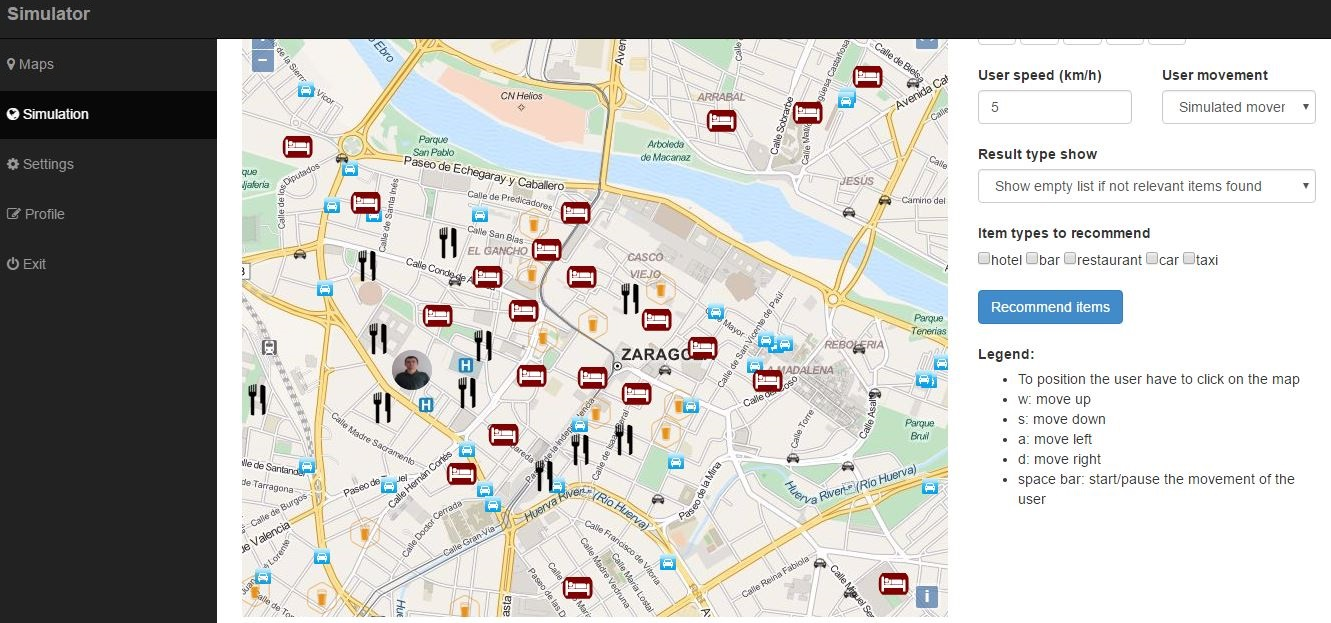
\includegraphics[scale=0.35]{imagenes/resumen-simulador.jpg}
\caption{Simulación en Actur, Zaragoza con un solo usuario}
\label{c2_trama}
\end{figure}

Puede ser usado a través de cualquier dispositivo (PC, tablet, móvil etc.) con conexión a Internet y un navegador web. Permite a los usuarios crear sus propios mapas y escenarios. Durante la creación de una escena el usuario elige cual es la cuidad donde se realiza la simulación, el recomendador a utilizar, si el mapa es colaborativo o no, introducir los objetos estáticos y configurar cuales son los objetos móviles y sus rutas. 

Para realizar una simulación el usuario tiene que buscar y seleccionar el mapa y escenario donde moverse tanto para obtener recomendaciones como para realizar votaciones sobre los distintos objetos de este entorno.

\section{Análisis de requisitos}

\subsection{Requisitos no funcionales}

\begin{table}[H]
	\begin{center}
		\begin{tabular}{|p{1.5cm}| p{10.5cm}|}
			\hline
			Código & Descripción \\
			\hline
			RNF-1  & La aplicación tratara de un simulador. Dicha simulación se realizara sobre mapas online\\ \hline
			RNF-2  & La navegación por los menús de la aplicación se realizara mediante una interfaz gráfica\\ \hline
			RNF-3  & Los textos por defecto de la aplicación serán en inglés\\ \hline
			RNF-4  & La autenfiticación de usuarios se realizará mediante web tokens\\ \hline
			RNF-5  & La interfaz gráfica debe ser responsive desarrollada con bootstrap\\ \hline
			RNF-6  & El back-end debe ser desarrollado con node.js, sockets.io y express \\ \hline
			RNF-7  & El front-end debe ser desarrollado con Angular.js\\ \hline
		\end{tabular}
		\caption{Requisitos no funcionales}
		\label{tabla:requisitosNoFuncionales}
	\end{center}
\end{table}

\newpage

\subsection{Requisitos funcionales}


\begin{longtable}[H]{|c|p{10cm}|}
	% aquí añadimos el encabezado de la primera hoja.
	\hline
	Código & Descripción \\
	\hline \hline
	\endfirsthead
	
	% aquí añadimos el encabezado del resto de hojas.
	\hline
	Código & Descripción \\
	\hline \hline
	\endhead
	
	% aquí añadimos el fondo de todas las hojas, excepto de la última.
	\multicolumn{2}{c}{}
	\endfoot
	
	% aquí añadimos el fondo de la última hoja.
	\endlastfoot
	
	% aquí añadimos el cuerpo de la tabla.
	RF-1  & La aplicación permitirá crear un nuevo usuario\\ \hline
	RF-2  & La aplicación permitirá al usuario buscar mapas por su nombre, tipo, estado, cuidad y fecha de creación\\ \hline
	RF-3  & La aplicación permitirá al usuario crear un nuevo mapa\\ \hline
	RF-4  & La aplicación permitirá al usuario crear una nueva escena asociada a un mapa existente\\ \hline
	RF-5  & La aplicación listara todas las escenas de un mapa\\ \hline
	RF-6  & La aplicación permitirá al usuario editar un mapa existente\\ \hline
	RF-7  & La aplicación permitirá al usuario editar las escenas de un mapa existente\\ \hline
	RF-8  & La aplicación permitirá al usuario crear un nuevo tipo de objeto estático\\ \hline
	RF-9  & La aplicación permitirá al usuario crear un nuevo tipo de objeto dinámico\\ \hline
	RF-10 & La aplicación listará todos los tipos de objetos estáticos creados\\ \hline
	RF-11 & La aplicación listará todos los tipos de objetos dinámicos creados\\ \hline
	RF-12 & La aplicación permitirá al usuario editar los objetos estáticos credos\\ \hline
	RF-13 & La aplicación permitirá al usuario editar los objetos dinámicos creados\\ \hline
	RF-14 & La aplicación permitirá al usuario cambiar el nombre\\ \hline
	RF-15 & La aplicación permitirá al usuario cambiar su contraseña\\ \hline
	RF-16 & La aplicación permitirá al usuario cambiar la imagen asociada a un usuario\\ \hline
	RF-17 & La aplicación permitirá al usuario configurar un nuevo tipo de recomendador\\ \hline
	RF-18 & La aplicación permitirá al usuario editar la configuración de recomendador existente\\ \hline
	RF-18 & La aplicación permitirá al usuario asociar un recomendador existente a una escena\\ \hline
	RF-19 & La aplicación permitirá al usuario definir los limites de una escena\\ \hline
	RF-20 & La aplicación permitirá al usuario asociar un objeto estático a una escena\\ \hline
	RF-21 & La aplicación permitirá al usuario cargar todos los objetos estáticos desde un fichero JSON\\ \hline
	RF-22 & La aplicación permitirá asociar un objeto dinámico y su definir su ruta en una escena\\ \hline
	RF-23 & La aplicación permitirá al usuario cargar todos los objetos dinámicos y sus rutas desde un fichero JSON\\ \hline
	RF-24 & La aplicación listará todos objetos estáticos asociados a una escena \\ \hline
	RF-25 & La aplicación listará todos los objetos dinámicos asociados a una escena \\ \hline
	RF-26 & La aplicación permitirá borrar un objeto estático asociado a una escena\\ \hline
	RF-27 & La aplicación permitirá borrar un objeto dinámico asociado a una escena\\ \hline
	RF-28 & La aplicación permitirá al usuario elegir un si mapa es colaborativo o no\\ \hline
	RF-29 & La aplicación permitirá al usuario ejecuta una simulación sobre la escena de un mapa\\ \hline
	RF-30 & La aplicación permitirá al usuario solicitar recomendaciones mientras se está ejecutando una simulación siempre y cuando el recomendador asociado a la escena es de tipo pull\\ \hline
	RF-31 & El usuario recibirá recomendaciones sin haberlas solicitado siempre y cuando el recomendador asociado a la escena de es tipo push\\ \hline
	RF-32 & El usuario puede arrancar/pausar una simulación\\ \hline
	RF-33 & La aplicación permitirá al usuario generar de forma aleatoria los grafos de movimiento de los vehículos \\ \hline	
	\caption{Requisitos funcionales}
	\label{tabla:requisitosFuncionales}
\end{longtable}

\newpage

\section{Arquitectura del sistema}

La arquitectura del sistema consta de cliente o navegador web, servidor web Node.js, servidor de recomendaciones y base de datos mongoDB (figura \ref{arquitecturaComponentes}).

El la figura \ref{arquitecturaComponentes} observamos que el navegador web se conecta al servidor Node.js mediante dos maneras: la primera es HTTP y la segunda es un sistema bidireccional dirigido por eventos. Las funcionalidades como creación de escenas, búsqueda de mapas etc. están desarrollados sobre una REST API y el intercambio de mensajes JSON.

El sistema bidireccional dirigido por eventos es utilizado  durante la simulación por una parte para reflejar los eventos generados por un usuario al resto de usuarios, y por otra para integrar el navegador, el servidor Node.js y el recomendador. De esta manera conseguimos compartir información entre los distintos componentes sin que estos los hayan solicitado evitando muchas peticiones innecesarias.

\begin{figure}[H]
\centering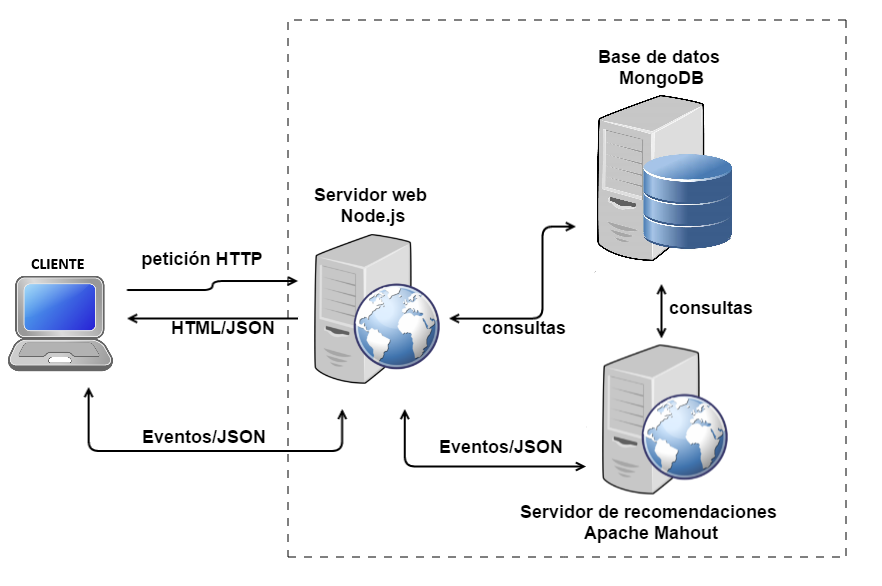
\includegraphics[scale=0.6]{imagenes/arquitectura-componentes.png}
\caption{Arquitectura de componentes del sistema}
\label{arquitecturaComponentes}
\end{figure}

\subsection{Arquitectura del front-end}

Para el desarrollo del front-end se han utilizado los frameworks Angular.js\footnote{framework que nos permite desarrollar aplicaciones de una sola página} y bootstrap\footnote{framework que nos ofrece un sistema de componentes reutilizables y adaptables a la pantalla del dispositivo}. Se ha decidido utilizar estas tecnologías porque nos ofrece varias ventajas: ahorro de recursos\footnote{angular.js va transmitiendo las vistas de la interfaz gráfica y las cachea al lado del cliente para ser reutilizadas posteriormente. Vuelve a solicitar una vista si y solo si esta ha sufrido algún cambio en el servidor}, mejora de la productividad y la posibilidad de realizar una simulación sobre dispositivos móviles\footnote{esto nos da la oportunidad de utilizar la posición geográfica del usuario para obtener recomendaciones en el entorno de una cuidad real. De está manera obtenemos datos reales y muchas más precisión a la hora de evaluar los algoritmos de recomendaciones} con el mismo código fuente.

La arquitectura del front-end está basada en el patrón Modelo-Vista-Controllador de tal forma que para cada vista existe un controlador que contiene la lógica de negocio de esta. El controlador también es el encargado de establecer comunicación con el back end. Esta comunicación se realiza entre los llamados Servicios\footnote{es pequeña fabrica de funciones y objetos inyectada en los controladores} de Angular.js y la REST API del back end. Los Servicios de Angular.js son muy necesarios y útiles ya que nos permiten crear un envoltorio sobre la REST API que nos ofrece el back end y de esta forma centralizar las llamas a la API.

\begin{figure}[H]
\centering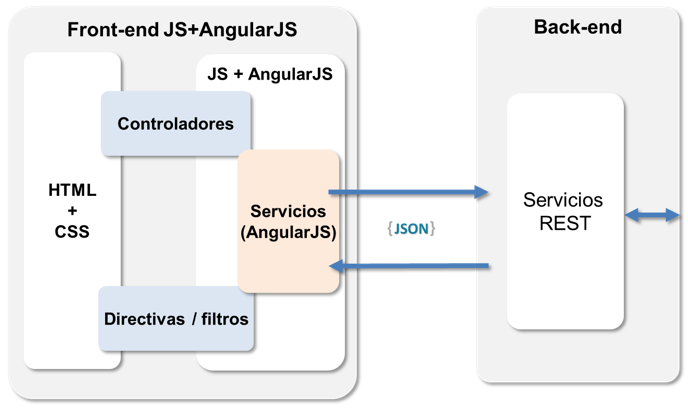
\includegraphics[scale=0.7]{imagenes/arquitectura-front-end.png}
\caption{Arquitectura del front-end}
\label{arquitecturaFrontEnd}
\end{figure}

\subsection{Arquitectura del back-end}


Para el desarrollo del back-end se han utilizado Node.js\footnote{javascript al lado del servidor}, Express\footnote{modulo de Node.js que nos ofrece la posibilidad de desarrollar una REST API}, socket.io\footnote{sistema bidireccional dirigido por eventos} y mongoose \footnote{modelado de objetos sobre mongoDB}. Se ha decidido utilizar estas tecnología por que nos ofrecen las siguientes ventajas: mejora la productividad a la hora de desarrollar el back-end, nos permite desarrollar un back-end ligero que consuma pocos recursos y el modulo sockets.io nos ofrece la posibilidad de desarrollar un sistema bidireccional dirigido por eventos.

La arquitectura del back-end se basa en la filosofía de desarrollo de aplicaciones con Node.js y Express y consiste de la siguiente estructura de directorios:

\dirtree{%
.1 Simulator.
.2 app.js.
.2 package.json.
.2 bin.
.3 www.
.2 models.
.2 public.
.3 images.
.3 javascript.
.4 angular.
.4 bootstrap.
.4 jquery.
.4 openlayers.
.4 socketIO.
.3 stylesheets.
.3 views.
.4 configurations.
.4 maps.
.4 settings.
.4 index.html.
.4 register.html.
.3 index.html.
.2 routes.
.3 configuratios.js.
.3 maps.js.
.3 simulation.js.
.3 user.js.
}

\newpage

A continuación vamos a ver más detalladamente cual es la función de cada elemento de este directorio:
\begin{itemize}
	\item app.js: centraliza las configuraciones de nuestra aplicación como por ejemplo en que puerto arranca el servidor, establecer conexiones con la base de datos, configuraciones del router\footnote{el router de Node.js es el encargado del direccionamiento de las peticiones y hace referencia a la definición de puntos finales de aplicación (URI) y cómo responden a las solicitudes de cliente} etc.
	\item package.json: es un gestor de paquetes y contiene los módulos que se están utilizando en nuestra aplicación.
	\item public: es un directorio que contiene la parte visual, es decir el front-end. Podemos ver que este contiene varios subdirectorios:
	\begin{itemize}
	\item en images se ubican las imágenes o iconos usados en la aplicación.
	\item en javascript se ubican los frameworks Javascript usados en en el front-end como Angular.js, Bootstrap, OpenLayers etc. En el subdirectorio angular podemos encontrar las configuraciones de Angular.js, los controladores de las vistas, los Servicios etc.
	\item en views se ubican las vistas del front-end.
	\item en stylesheets están ubicadas las hojas de estilos
	\end{itemize}
	\item en routes se ubican las distintas rutas de Express. En nuestro caso tenemos una para cada menú de la aplicación. Por ejemplo todas las operaciones referentes al menú Maps se encuentra en el fichero maps.js etc.
\end{itemize}

\subsection{Arquitectura de recomendador}

El desarrollo del recomendador está realizado con Java 7, la librería Apache Mahout y socket.io-client. El recomendador desarrollado es un recomendador pull\footnote{tipo de recomendador en el cual los usuarios solicitan recomendaciones} de ejemplo basado en los usuarios (User based recommender). 

Aunque sea un recomendador de ejemplo este está pensado para se expandido, tanto para otro tipo de recomendadores (como pueden ser los recomendadores de tipo push\footnote{tipo de recomendador que realiza recomendaciones sin que el usuario los haya solicitado}) como para la implementación de nuevos tipos de estrategias para el recomendador de tipo pull.

Durante el arranque el servidor del recomendador lanza un hilo por cada tipo de recomendador. En nuestro caso solo lanza un hilo que se corresponde al servidor de tipo pull. Este hilo es el que contiene los eventos que invoca el simulador de escenarios. En la figura \ref{diagramaEventos} observamos que tenemos solo dos eventos: uno para recuperar los tipos de implementaciones\footnote{en nuestro caso es User based recommender pero existen otros tipos como Item based recommender} y otro para realizar las recomendaciones.

\begin{figure}[H]
\centering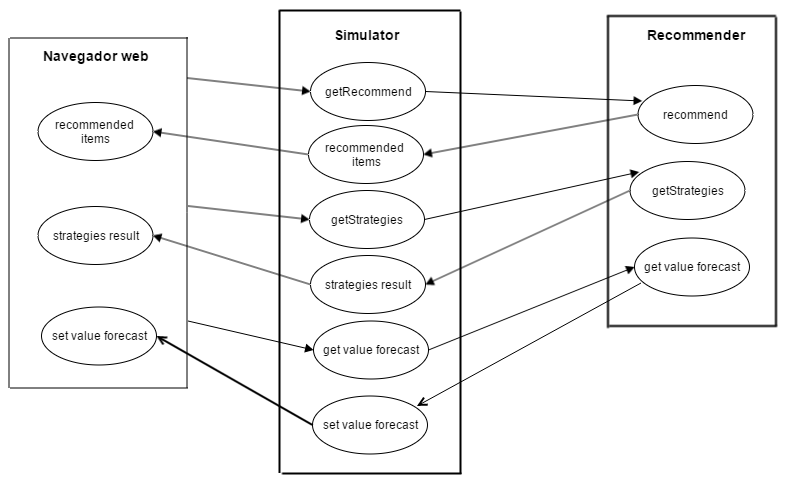
\includegraphics[scale=0.6]{imagenes/diagrama-de-eventos.png}
\caption{Diagrama de eventos}
\label{diagramaEventos}
\end{figure}

El evento recommend es el que se dispara cuando uno de los usuarios solicita una recomendación. Para que se puedan utilizar distintos tipos de implementaciones del recomendador de tipo pull se ha implementado un patrón de diseño de tipo Strategy. Este patrón de diseños nos permite cambiar de estrategia de recomendación en tiempo de ejecución:

\begin{figure}[H]
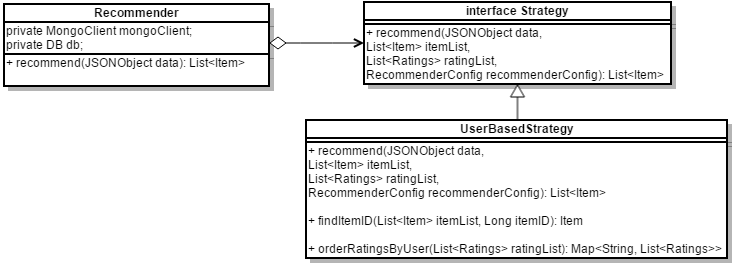
\includegraphics[scale=0.7]{imagenes/uml.png}
\caption{Diagrama uml del patrón de diseño de tipo Strategy}
\label{diagramaUMLStrategy}
\end{figure}

\subsection{Autentificación Basada en Token}

La autentificación es una de las partes más importantes de un sistema. En este desarrollo se ha optado por una autentificación basada en token. En la autentificación basada en token, las cookies y las sesiones no se utilizan. Se emplea un token para autentificar al usuario en cada petición que se hace al servidor. El flujo de control es el siguiente:
\begin{enumerate}[1.]
	\item el usuario provee un nombre de usuario y contraseña en el formulario de login.
	\item una vez hecha la petición, se valida el usuario en el back-end mediante una consulta a la base de datos. Si la petición es válida, se crea un token utilizando la información de usuario brindada por la base de datos, y luego se retorna esa información en el encabezado de la respuesta, para así guardar el token en almacenamiento local.
	\item se provee la información del token en el encabezado de cada petición para acceder a endpoints restringidos de la aplicación.
	\item si el token tomado del encabezado de la petición es válido, se permite al usuario acceder al endpoint especificado, y se responde con JSON o HTML.
\end{enumerate}

\begin{figure}[H]
	\centering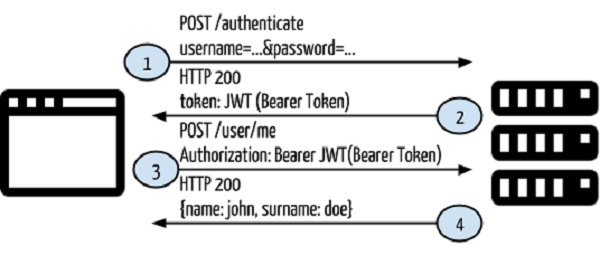
\includegraphics[scale=0.7]{imagenes/token.png}
	\caption{Autentificación Basada en Token}
	\label{token}
\end{figure}

\newpage

\subsubsection{Estructura de un token}

Un token consiste de tres partes:
\begin{itemize}
	\item encabezado: es la parte del token que almacena el tipo de token y el método de encriptación, que a su vez está encriptado en base-64.
	\item carga útil: incluye la información que queremos encriptar.
	\item firma: consiste de combinaciones del encabezado, carga útil, y clave secreta. La clave secreta debe ser almacenada del lado servidor.
\end{itemize}

\begin{figure}[H]
	\centering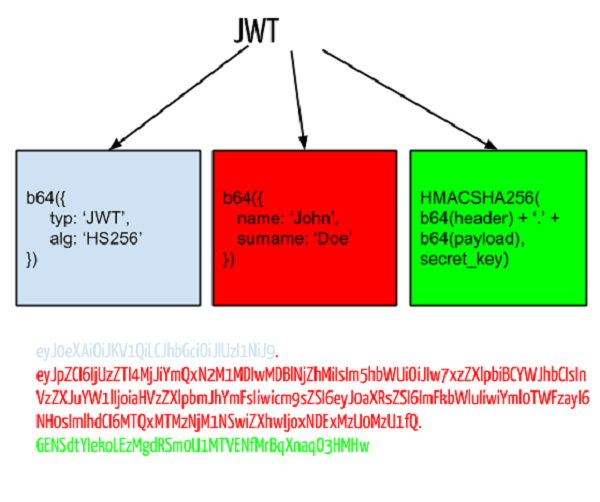
\includegraphics[scale=0.5]{imagenes/jwt.png}
	\caption{Formato del Token}
	\label{formatoToken}
\end{figure}

\section{Menús del simulador de escenarios}

Como en todas las aplicaciones, el simulador de escenarios cuenta con un sistema de menús que dan acceso a las distintas opciones del simulador. En este caso se ha seguido la paradigma WIMP para la organización de los menús y distintas opciones (figura \ref{mapaNavegacion}). Existen 4 tipos de caminos organizados en forma de árbol:

\begin{itemize}
	\item busqueda y gestión (creación, edición y borrados) de mapas y escenas
	\item simulación de un mapa y escena
	\item gestión de tipos de recomendadores, objetos estáticos\footnote{objetos que no cambian de posición a medida que pasa el tiempo} y dinámicos\footnote{objetos que cambian de posición a medida que pasa el tiempo. Tienen una ruta definida durante la creación de la escena}
	\item configuraciones del perfil del usuario
\end{itemize} 

\begin{figure}[H]
\centering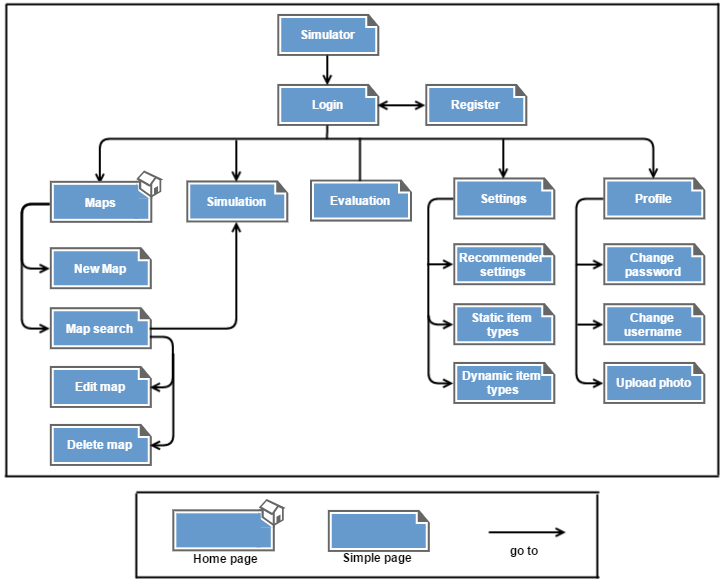
\includegraphics[scale=0.7]{imagenes/mapa-navegacion.png}
\caption{Mapa de navegación}
\label{mapaNavegacion}
\end{figure}

\newpage

\section{Navegación por estima}

La navegación por estima es una técnica que se aplica en el cliente. Consiste en procesar en cada ciclo el estado de los objetos móviles. Se trata de una técnica analítica utilizada en la náutica para la navegación y situación de los barcos y se tienen en cuenta los siguientes elementos: la situación actual, rumbo y velocidad. Es decir, sabiendo la velocidad, el rumbo de la nave y el tiempo transcurrido se puede estimar la posición de la misma al cabo del tiempo. 

Con este método conseguimos calcular cual es la siguiente posición geográfica donde tenemos que colocar un objeto móvil al acabo de un tiempo (el tiempo de refresco de la pantalla). Como ventaja conseguimos disminuir el error en el cálculo de las posiciones de los objetos móviles. Así obtenemos movimientos muy precisos incluso en grafos de movimientos con nodos muy cercanos.

\section{Diseño final}

En esta sección se dejan solo algunas de las pantallas más relevantes de la aplicación. Para ver más pantallas debe acudir al manual de usuario en los anexos.

\begin{figure}[H]
 \centering
  \subfloat[Autentificación de un usuario]{
   \label{f:login}
    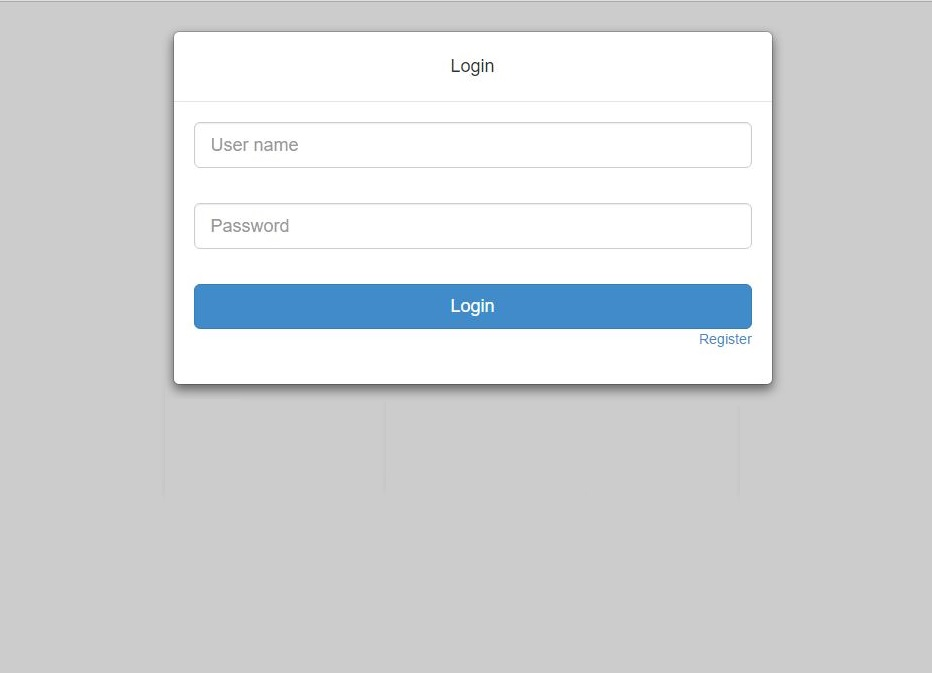
\includegraphics[width=0.5\textwidth]{imagenes/login.jpg}}
  \subfloat[Crear un nuevo usuario]{
   \label{f:register}
    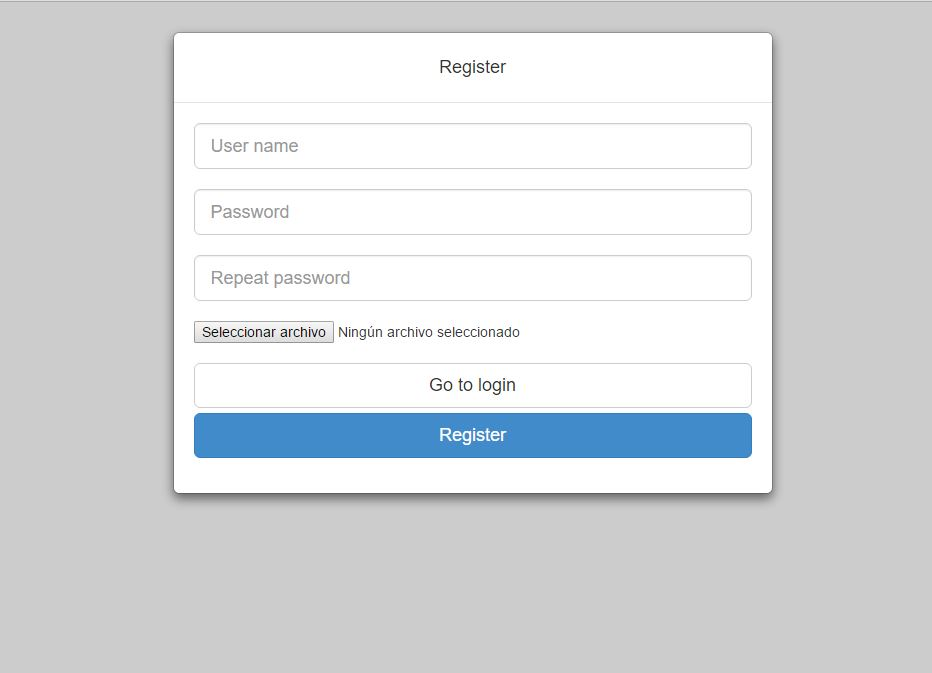
\includegraphics[width=0.5\textwidth]{imagenes/register.jpg}}
 \caption{Registro y autentificación de un usuario}
 \label{f:LoginRegister}
\end{figure}

\begin{figure}[H]
\centering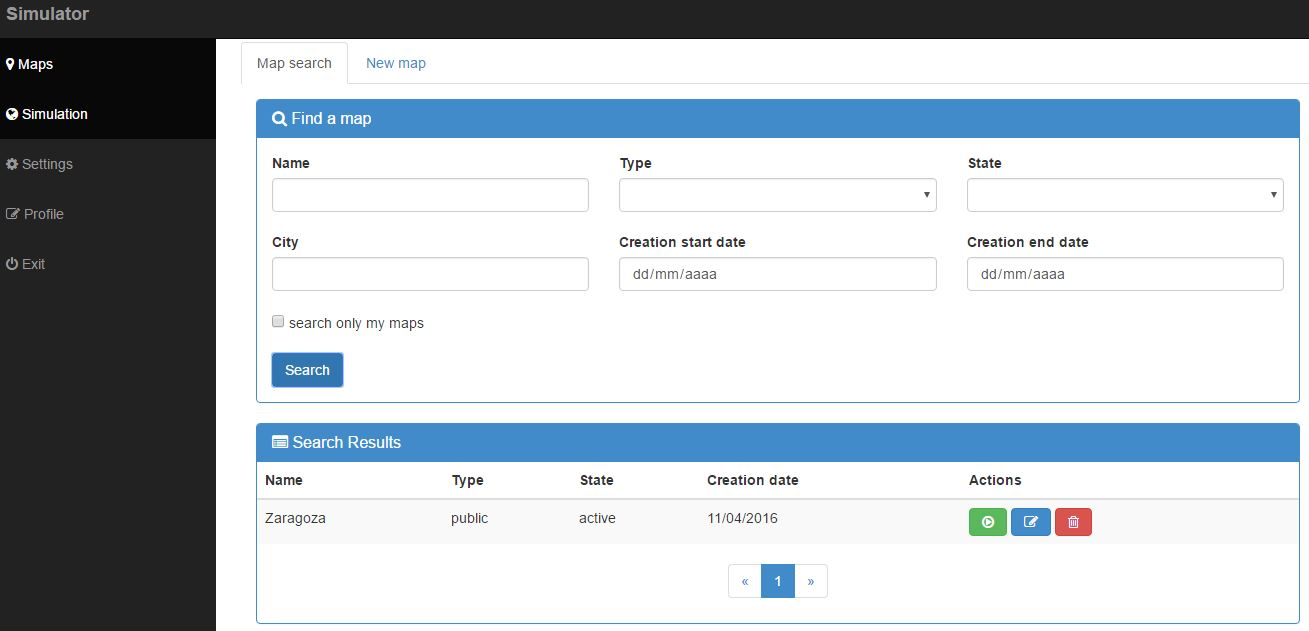
\includegraphics[scale=0.3]{imagenes/busqueda-de-mapas.jpg}
\caption{Busqueda de mapas}
\label{BusquedaMapas}
\end{figure}

\begin{figure}[H]
\centering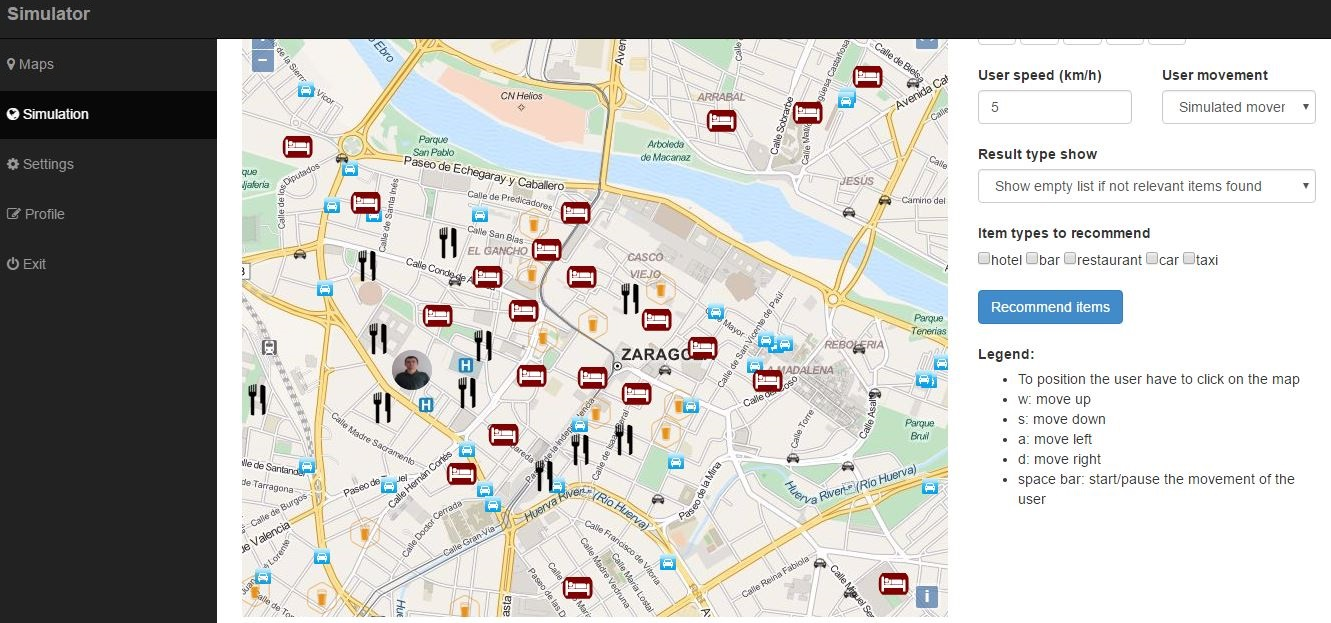
\includegraphics[scale=0.3]{imagenes/resumen-simulador.jpg}
\caption{Simulación en Actur, Zaragoza}
\label{simulacionActur}
\end{figure}

\begin{figure}[H]
\centering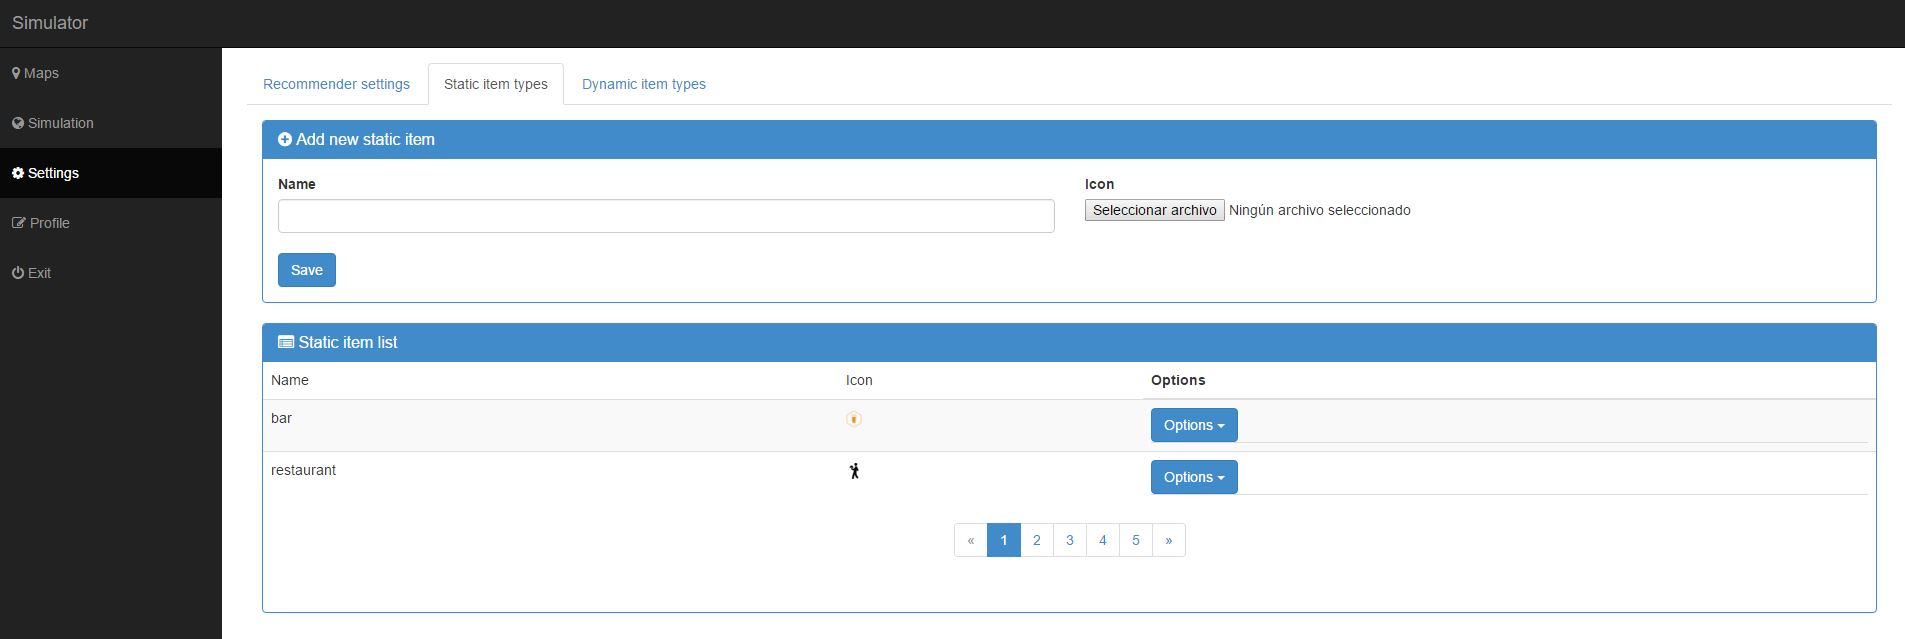
\includegraphics[scale=0.3]{imagenes/config-objetos-estaticos.jpg}
\caption{Configuración de los objetos estáticos}
\label{ConfigStaticItem}
\end{figure}